\documentclass[aspectratio=169,12pt]{beamer}
\usetheme{Madrid}
\usecolortheme{default}
\usepackage[utf8]{inputenc}
\usepackage[T1]{fontenc}
\usepackage{graphicx}
\usepackage{tikz}
\usepackage{xcolor}
\usepackage{multicol}
\usepackage{booktabs}
\usepackage{amssymb}

\usetikzlibrary{shapes.geometric, arrows, positioning, shadows, backgrounds, fit, calc, shapes.symbols}

% Custom colors
\definecolor{euroblue}{RGB}{0,51,153}
\definecolor{eurogold}{RGB}{255,204,0}
\definecolor{warningred}{RGB}{220,20,60}
\definecolor{safegreen}{RGB}{34,139,34}
\definecolor{cautionorange}{RGB}{255,140,0}

% Title page information
\title[European AI Regulation]{The European Artificial Intelligence Act}
\subtitle{A Comprehensive Framework for AI Governance}
\author{Prof. Fedeli Massimo - Tutti i diritti riservati}
\institute{IIS Fermi Sacconi Cpia - Ascoli Piceno}
\date{\today}

\begin{document}

% Title slide
\begin{frame}
\titlepage
\begin{center}
\begin{tikzpicture}[remember picture,overlay]
\node[opacity=0.1] at (current page.center) {\includegraphics[width=0.4\textwidth]{example-image}};
\end{tikzpicture}
\end{center}
\end{frame}

% Slide 1: Introduction
\begin{frame}{The AI Revolution in Our Daily Lives}
\begin{columns}[T]
\column{0.55\textwidth}
\textbf{AI is everywhere:}
\begin{itemize}
\item Online recommendations and suggestions
\item Voice assistants on smartphones
\item Credit evaluation systems
\item CV screening for job applications
\item Social media content filtering
\end{itemize}

\vspace{0.3cm}
\textbf{The need for regulation:}
\begin{itemize}
\item Protect fundamental rights
\item Ensure safety and transparency
\item Balance innovation with protection
\end{itemize}

\column{0.4\textwidth}
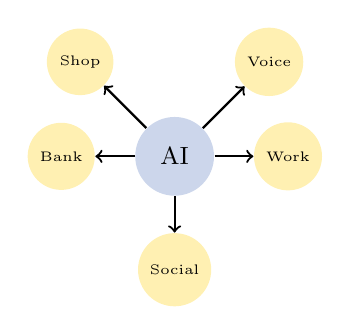
\begin{tikzpicture}[scale=0.8]
% Draw interconnected AI applications
\node[circle, fill=euroblue!20, minimum size=1cm] (center) at (0,0) {\small AI};
\node[circle, fill=eurogold!30, minimum size=0.8cm] (app1) at (-1.5,1.5) {\tiny Shop};
\node[circle, fill=eurogold!30, minimum size=0.8cm] (app2) at (1.5,1.5) {\tiny Voice};
\node[circle, fill=eurogold!30, minimum size=0.8cm] (app3) at (-1.8,0) {\tiny Bank};
\node[circle, fill=eurogold!30, minimum size=0.8cm] (app4) at (1.8,0) {\tiny Work};
\node[circle, fill=eurogold!30, minimum size=0.8cm] (app5) at (0,-1.8) {\tiny Social};

\draw[thick, ->] (center) -- (app1);
\draw[thick, ->] (center) -- (app2);
\draw[thick, ->] (center) -- (app3);
\draw[thick, ->] (center) -- (app4);
\draw[thick, ->] (center) -- (app5);
\end{tikzpicture}
\end{columns}
\end{frame}

% Slide 2: The AI Act - Key Facts
\begin{frame}{The AI Act: A Historic Achievement}
\begin{tikzpicture}[remember picture,overlay]
\node[anchor=north east, opacity=0.05] at (current page.north east) {\includegraphics[width=0.3\textwidth]{example-image}};
\end{tikzpicture}

\begin{block}{Key Milestones}
\begin{itemize}
\item \textbf{December 9, 2023}: Provisional agreement reached
\item \textbf{First in the world}: Comprehensive AI regulatory framework
\item \textbf{Landmark legislation}: Sets global standards for AI governance
\end{itemize}
\end{block}

\vspace{0.5cm}

\begin{columns}[T]
\column{0.5\textwidth}
\textbf{What it defines:}
\begin{itemize}
\item What can and cannot be done with AI
\item Guarantees for citizens
\item Responsibilities for companies
\end{itemize}

\column{0.5\textwidth}
\textbf{Who it affects:}
\begin{itemize}
\item AI developers and providers
\item Companies using AI systems
\item Public institutions
\item Citizens and end users
\end{itemize}
\end{columns}
\end{frame}

% Slide 3: Risk-Based Approach
\begin{frame}{An Innovative Approach: Risk-Based Regulation}
\begin{center}
\textbf{\Large The fundamental principle:}\\
\vspace{0.3cm}
\textit{``Higher risk = Stricter rules''}
\end{center}

\vspace{0.5cm}

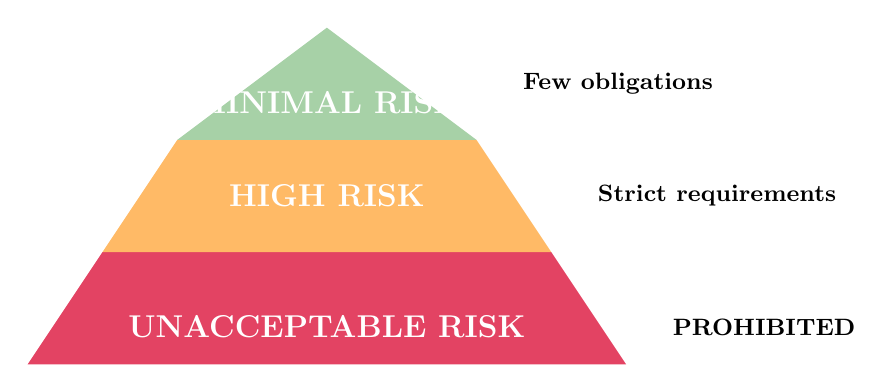
\begin{tikzpicture}[scale=0.95, transform shape]
% Draw pyramid showing risk levels
\fill[warningred!80] (0,0) -- (8,0) -- (7,1.5) -- (1,1.5) -- cycle;
\fill[cautionorange!60] (1,1.5) -- (7,1.5) -- (6,3) -- (2,3) -- cycle;
\fill[safegreen!40] (2,3) -- (6,3) -- (4,4.5) -- cycle;

% Labels
\node[white, font=\large\bfseries] at (4,0.5) {UNACCEPTABLE RISK};
\node[white, font=\large\bfseries] at (4,2.25) {HIGH RISK};
\node[white, font=\large\bfseries] at (4,3.5) {MINIMAL RISK};

% Side annotations
\node[anchor=west, font=\small] at (8.5,0.5) {\textbf{PROHIBITED}};
\node[anchor=west, font=\small] at (7.5,2.25) {\textbf{Strict requirements}};
\node[anchor=west, font=\small] at (6.5,3.75) {\textbf{Few obligations}};
\end{tikzpicture}

\vspace{0.3cm}
\begin{center}
\small \textit{Finding the balance between protection and innovation}
\end{center}
\end{frame}

% Slide 4: Unacceptable Risk - Prohibited Practices
\begin{frame}{Unacceptable Risk: Prohibited AI Practices}
\begin{tikzpicture}[remember picture,overlay]
\node[anchor=north west, text=warningred, font=\Huge] at ([xshift=1cm,yshift=-1cm]current page.north west) {$\times$};
\end{tikzpicture}

\textbf{These AI applications are completely banned in the EU:}

\begin{enumerate}
\item \textbf{Behavioral manipulation systems}
   \begin{itemize}
   \item Exploiting vulnerabilities (age, disability, economic status)
   \item Subliminal or deceptive techniques
   \end{itemize}

\item \textbf{Social scoring systems}
   \begin{itemize}
   \item Rating citizens based on behavior or characteristics
   \item Mass social surveillance by public or private entities
   \end{itemize}

\item \textbf{Biometric categorization based on sensitive data}
   \begin{itemize}
   \item Inferring race, political opinions, sexual orientation
   \item Deducing religious or philosophical beliefs
   \end{itemize}
\end{enumerate}

\vspace{0.2cm}
\begin{alertblock}{Principle}
These practices are incompatible with EU fundamental values and the Charter of Fundamental Rights.
\end{alertblock}
\end{frame}



% Slide 5: More Prohibited Practices
\begin{frame}{More Prohibited Practices}
\begin{columns}[T]
\column{0.48\textwidth}
\begin{block}{4. Emotion Recognition}
\textbf{Prohibited in:}
\begin{itemize}
\item Workplace environments
\item Educational institutions
\end{itemize}
\textbf{Exception:}
\begin{itemize}
\item Medical and safety purposes
\item Example: monitoring pilot fatigue
\end{itemize}
\end{block}

\end{columns}
\end{frame}

\begin{frame}{More Prohibited Practices}
\begin{block}{5. Facial Image Scraping}
	\begin{itemize}
		\item Untargeted collection from internet
		\item From CCTV systems
		\item To create/expand facial recognition databases
	\end{itemize}
\end{block}
\end{frame}


\begin{frame}{More Prohibited Practices}
	\begin{columns}[T]
	\column{0.48\textwidth}
	\begin{block}{6. Real-Time Facial Recognition}
		\textbf{General prohibition} for law enforcement in public spaces
		
		\vspace{0.2cm}
		\textbf{Limited exceptions:}
		\begin{itemize}
			\item Targeted search for victims
			\item Prevention of specific threats
			\item Detection of serious crimes
		\end{itemize}
		
		\vspace{0.2cm}
		\textit{Requires judicial authorization and strict oversight}
	\end{block}
	
	
\begin{tikzpicture}
		\node[cloud, draw, fill=warningred!20, cloud puffs=10, minimum width=3cm, minimum height=1.5cm, align=center] {Privacy\\Protection};
	\end{tikzpicture}
	\end{columns}
\end{frame}


% NEW SLIDE 6: Concrete Example - Emotion Recognition
\begin{frame}{Concrete Example: Emotion Recognition Ban}
	\begin{columns}[T]
		\column{0.48\textwidth}
		\begin{alertblock}{Prohibited Scenario}
			\textbf{Company X installs emotion detection cameras}
			\begin{itemize}
				\item Monitors employee facial expressions
				\item Analyzes engagement levels during meetings
				\item Uses data for performance evaluations
				\item Claims to detect stress or happiness
			\end{itemize}
			\vspace{0.2cm}
			\textbf{Result:} \textcolor{warningred}{PROHIBITED}
		\end{alertblock}
		

		\column{0.48\textwidth}
		\begin{block}{School Example}
			\textbf{University installs AI to detect student attention}
			\begin{itemize}
				\item Cameras analyze facial expressions
				\item System flags distracted students
				\item Data shared with professors
				\item Affects participation grades
			\end{itemize}
			\vspace{0.2cm}
			\textbf{Result:} \textcolor{warningred}{PROHIBITED}
		\end{block}

	\end{columns}
\end{frame}

% NEW SLIDE 7: Social Scoring Example
\begin{frame}{Concrete Example: Social Scoring Systems}
\begin{alertblock}{Prohibited: CitizenScore System}
\textbf{City government implements AI scoring:}
\begin{itemize}
\item Tracks social media, shopping, social connections
\item Assigns score 0-1000 to each citizen
\item High scorers: priority housing, faster permits
\item Low scorers: service restrictions, higher rates
\end{itemize}
\vspace{0.2cm}
\textbf{Result:} \textcolor{warningred}{\Large ABSOLUTELY PROHIBITED}
\end{alertblock}

\begin{columns}[T]
\column{0.48\textwidth}
\begin{block}{Why Banned}
\begin{itemize}
\item Mass surveillance
\item Discriminatory access
\item Chills free expression
\item Violates human dignity
\item Creates social control
\end{itemize}
\end{block}

\column{0.48\textwidth}
\begin{block}{Real Context}
\textbf{China's Social Credit:}
\begin{itemize}
\item Millions affected
\item Restricts travel, jobs
\item Based on behavior tracking
\end{itemize}
\vspace{0.3cm}
\textit{Such systems CANNOT exist in EU}
\end{block}
\end{columns}
\end{frame}

% NEW SLIDE 8: Biometric Violations
\begin{frame}{Concrete Examples: Biometric Violations}
\begin{columns}[T]
\column{0.48\textwidth}
\begin{alertblock}{Prohibited: Biometric Categorization}
\textbf{Airport Security System}
\begin{itemize}
\item AI analyzes facial features
\item Infers ethnicity, religion
\item Flags profiles for screening
\item Appearance-based only
\end{itemize}
\vspace{0.2cm}
\textbf{Result:} \textcolor{warningred}{PROHIBITED}
\end{alertblock}

\begin{alertblock}{Prohibited: Facial Scraping}
\textbf{Tech Company Database}
\begin{itemize}
\item Scrapes billions of photos
\item Builds facial recognition DB
\item Sells to companies
\item No user consent
\end{itemize}
\vspace{0.2cm}
\textbf{Result:} \textcolor{warningred}{PROHIBITED}
\end{alertblock}

\column{0.48\textwidth}
\begin{block}{Case Study: Clearview AI}
\begin{itemize}
\item US company: 3+ billion images
\item Sold to law enforcement
\item EU countries fined them
\item \textbf{AI Act explicitly bans this}
\end{itemize}
\end{block}

\begin{exampleblock}{The Harm}
\begin{itemize}
\item Violates privacy massively
\item Enables discrimination
\item No individual control
\item Perpetuates biases
\item Chills freedom
\end{itemize}
\end{exampleblock}

\vspace{0.3cm}
\textit{Your face is not free data}
\end{columns}
\end{frame}

\begin{frame}{High-Risk AI Systems: When AI Needs Special Safeguards}
\begin{tikzpicture}[remember picture,overlay]
\node[anchor=north east, text=cautionorange, font=\Huge] at ([xshift=-1cm,yshift=-1cm]current page.north east) {$\triangle$!};
\end{tikzpicture}

\textbf{Not prohibited, but requiring strict obligations}

\vspace{0.4cm}

\begin{columns}[T]
\column{0.48\textwidth}
\begin{block}{Key Requirements}
\begin{itemize}
\item Conformity assessment before market release
\item Quality data for training
\item Technical documentation
\item Transparency of operation
\item Human oversight capability
\item Accuracy and robustness
\item Cybersecurity measures
\end{itemize}
\end{block}

\column{0.48\textwidth}
\begin{block}{Main Principle}
Systems can be used only if they meet quality, safety, and transparency standards
\end{block}

\vspace{0.3cm}

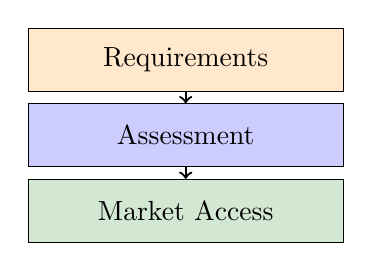
\begin{tikzpicture}[scale=0.8]
\node[rectangle, draw, fill=cautionorange!20, minimum width=4cm, minimum height=0.8cm] (req) at (0,0) {Requirements};
\node[rectangle, draw, fill=blue!20, minimum width=4cm, minimum height=0.8cm] (assess) at (0,-1.2) {Assessment};
\node[rectangle, draw, fill=safegreen!20, minimum width=4cm, minimum height=0.8cm] (market) at (0,-2.4) {Market Access};

\draw[->, thick] (req) -- (assess);
\draw[->, thick] (assess) -- (market);
\end{tikzpicture}
\end{columns}
\end{frame}

% Slide 7: Training Data Requirements
\begin{frame}{Data Quality: Fighting Discrimination}
\textbf{High-risk systems must be trained with representative datasets}

\vspace{0.5cm}

\begin{example}[Problem: Biased Recruitment System]
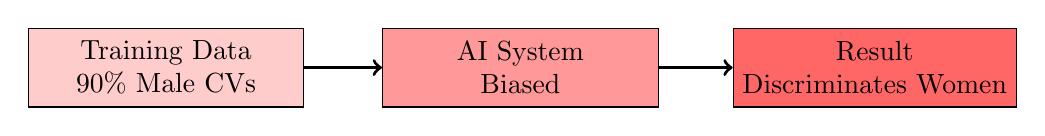
\begin{tikzpicture}[scale=0.9]
% Biased training
\node[rectangle, draw, fill=red!20, minimum width=3.5cm, minimum height=1cm, align=center] (bias) at (0,0) {Training Data\\90\% Male CVs};
\node[rectangle, draw, fill=red!40, minimum width=3.5cm, minimum height=1cm, align=center] (ai) at (5,0) {AI System\\Biased};
\node[rectangle, draw, fill=red!60, minimum width=3.5cm, minimum height=1cm, align=center] (result) at (10,0) {Result\\Discriminates Women};

\draw[->, very thick] (bias) -- (ai);
\draw[->, very thick] (ai) -- (result);
\end{tikzpicture}
\end{example}

\vspace{0.5cm}

\begin{exampleblock}{Solution: Representative Training}
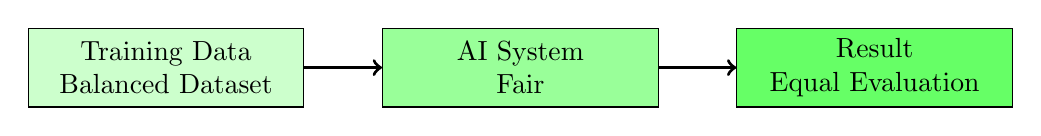
\begin{tikzpicture}[scale=0.9]
% Balanced training
\node[rectangle, draw, fill=green!20, minimum width=3.5cm, minimum height=1cm, align=center] (good) at (0,0) {Training Data\\Balanced Dataset};
\node[rectangle, draw, fill=green!40, minimum width=3.5cm, minimum height=1cm, align=center] (ai2) at (5,0) {AI System\\Fair};
\node[rectangle, draw, fill=green!60, minimum width=3.5cm, minimum height=1cm, align=center] (result2) at (10,0) {Result\\Equal Evaluation};

\draw[->, very thick] (good) -- (ai2);
\draw[->, very thick] (ai2) -- (result2);
\end{tikzpicture}
\end{exampleblock}

\vspace{0.3cm}
\begin{center}
\textbf{The regulation requires identification and mitigation of discrimination risks}
\end{center}
\end{frame}

% Slide 8: Traceability and Transparency
\begin{frame}{Traceability: Understanding AI Decisions}
\begin{block}{Why Traceability Matters}
High-risk systems must be traceable to reconstruct:
\begin{itemize}
\item How the system reached a decision
\item Which data were used
\item How the system was trained
\end{itemize}
\end{block}

\vspace{0.5cm}

\begin{center}
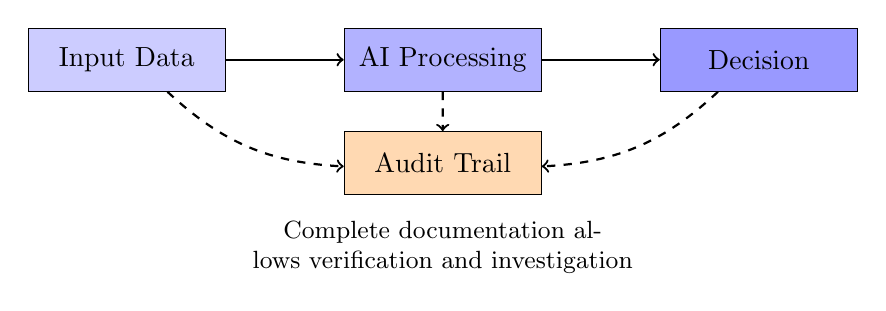
\begin{tikzpicture}[scale=0.85, node distance=1.5cm]
\node[rectangle, draw, fill=blue!20, minimum width=2.5cm, minimum height=0.8cm] (input) {Input Data};
\node[rectangle, draw, fill=blue!30, minimum width=2.5cm, minimum height=0.8cm, right=of input] (process) {AI Processing};
\node[rectangle, draw, fill=blue!40, minimum width=2.5cm, minimum height=0.8cm, right=of process] (output) {Decision};
\node[rectangle, draw, fill=orange!30, minimum width=2.5cm, minimum height=0.8cm, below=0.5cm of process] (trace) {Audit Trail};

\draw[->, thick] (input) -- (process);
\draw[->, thick] (process) -- (output);
\draw[->, thick, dashed] (process) -- (trace);
\draw[->, thick, dashed] (input) to[bend right=20] (trace);
\draw[->, thick, dashed] (output) to[bend left=20] (trace);

\node[below=0.2cm of trace, font=\small, text width=8cm, align=center] {Complete documentation allows verification and investigation};
\end{tikzpicture}
\end{center}
\end{frame}

% Slide 9: Categories of High-Risk Systems - Part 1
\begin{frame}{High-Risk Systems: Practical Categories (1/2)}
\begin{columns}[T]
\column{0.48\textwidth}
\begin{block}{1. Biometric Identification}
\begin{itemize}
\item Biometric systems for identifying people
\item When not completely prohibited
\item Strict oversight required
\end{itemize}
\end{block}

\begin{block}{2. Critical Infrastructure}
\begin{itemize}
\item Electricity, water, gas networks
\item Road traffic management
\item Systems whose failure could impact safety
\end{itemize}
\end{block}

\begin{block}{3. Education}
\begin{itemize}
\item Determining access to institutions
\item Evaluating learning outcomes
\item Monitoring for exam dishonesty
\end{itemize}
\end{block}

\column{0.48\textwidth}
\begin{block}{4. Employment}
\begin{itemize}
\item CV screening systems
\item Interview evaluation
\item Performance monitoring
\item Promotion and dismissal decisions
\end{itemize}
\end{block}

\vspace{0.5cm}

\begin{alertblock}{Common Thread}
All these systems can significantly affect people s fundamental rights and safety
\end{alertblock}
\end{columns}
\end{frame}

% Slide 10: Categories of High-Risk Systems - Part 2
\begin{frame}{High-Risk Systems: Practical Categories (2/2)}
\begin{columns}[T]
\column{0.48\textwidth}
\begin{block}{5. Essential Services}
\begin{itemize}
\item Access to public benefits
\item Healthcare access
\item Social welfare eligibility
\item Emergency services dispatch
\end{itemize}
\end{block}

\begin{block}{6. Financial Services}
\begin{itemize}
\item Credit scoring systems
\item Creditworthiness evaluation
\item Insurance premium calculation
\item Loan approval decisions
\end{itemize}
\end{block}

\column{0.48\textwidth}
\begin{block}{7. Justice and Law (Italian Request)}
\begin{itemize}
\item Assisting judges in research
\item Interpretation of facts and law
\item Alternative dispute resolution
\end{itemize}
\vspace{0.2cm}
\small \textit{Italy successfully advocated for including judicial AI systems}
\end{block}

\vspace{0.3cm}

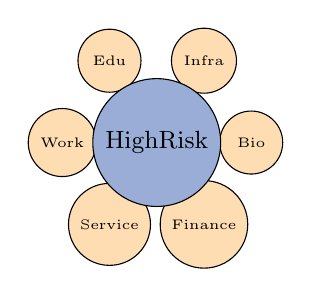
\begin{tikzpicture}[scale=0.8]
\foreach \angle/\label in {0/Bio, 60/Infra, 120/Edu, 180/Work, 240/Service, 300/Finance} {
    \node[circle, draw, fill=cautionorange!30, minimum size=0.8cm, font=\tiny] at (\angle:1.5) {\label};
}
\node[circle, draw, fill=euroblue!40, minimum size=1cm, font=\small] at (0,0) {High\\Risk};
\end{tikzpicture}
\end{columns}
\end{frame}

% Slide 11: Fundamental Rights Impact Assessment
\begin{frame}{Fundamental Rights Impact Assessment}
\textbf{Additional obligation for public entities and public service providers}

\vspace{0.5cm}

\begin{block}{The Assessment Must Describe:}
\begin{enumerate}
\item How the system will be used
\item Who will be affected by it
\item What risks exist
\item What mitigation measures have been adopted
\end{enumerate}
\end{block}

\vspace{0.5cm}

\begin{center}
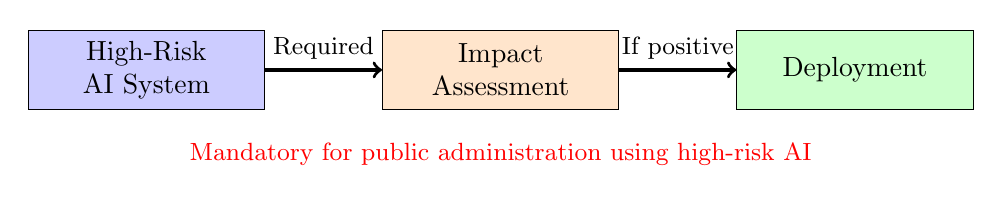
\begin{tikzpicture}[scale=0.9]
\node[rectangle, draw, fill=blue!20, minimum width=3cm, minimum height=1cm, align=center] (system) at (0,0) {High-Risk\\AI System};
\node[rectangle, draw, fill=orange!20, minimum width=3cm, minimum height=1cm, align=center] (assess) at (5,0) {Impact\\Assessment};
\node[rectangle, draw, fill=green!20, minimum width=3cm, minimum height=1cm, align=center] (deploy) at (10,0) {Deployment};

\draw[->, very thick] (system) -- node[above, font=\small] {Required} (assess);
\draw[->, very thick] (assess) -- node[above, font=\small] {If positive} (deploy);

\node[below=0.3cm of assess, text width=10cm, align=center, font=\small, text=red] {Mandatory for public administration using high-risk AI};
\end{tikzpicture}
\end{center}
\end{frame}

% Slide 12: Minimal Risk Systems
\begin{frame}{Minimal Risk: The Majority of AI Systems}
\begin{tikzpicture}[remember picture,overlay]
\node[anchor=north east, text=safegreen, font=\Huge] at ([xshift=-1cm,yshift=-1cm]current page.north east) {$\checkmark$};
\end{tikzpicture}

\textbf{Most AI systems currently used in the EU fall into this category}

\vspace{0.5cm}

\begin{columns}[T]
\column{0.48\textwidth}
\begin{block}{Examples}
\begin{itemize}
\item Video games with AI
\item Spam filters
\item Online shopping recommendations
\item Many everyday applications
\end{itemize}
\end{block}

\begin{block}{Requirements}
\begin{itemize}
\item No special obligations
\item No conformity assessments
\item No complex bureaucracy
\end{itemize}
\end{block}

\column{0.48\textwidth}
\begin{block}{Voluntary Measures}
Encouraged adoption of:
\begin{itemize}
\item Codes of conduct
\item Best practices
\item Self-regulation
\end{itemize}
\end{block}

\vspace{0.3cm}

\begin{block}{Integration}
Systems already regulated by:
\begin{itemize}
\item Digital Services Act (DSA)
\item Digital Markets Act (DMA)
\end{itemize}
No regulatory overlap
\end{block}
\end{columns}

\vspace{0.3cm}
\begin{center}
\textbf{Focus: Not stifling innovation while maintaining basic standards}
\end{center}
\end{frame}

% Slide 13: Transparency Requirements
\begin{frame}{Transparency: The Right to Know}
\textbf{Users must be informed when interacting with AI}

\vspace{0.5cm}

\begin{columns}[T]
\column{0.48\textwidth}
\begin{block}{1. Chatbots and Virtual Assistants}
Clear disclosure required:
\begin{itemize}
\item User is interacting with a machine
\item Not a real person
\item Prevents deception
\end{itemize}
\end{block}

\begin{example}[Good Practice]
\textit{``Hello! I'm an AI assistant. How can I help you today?''}
\end{example}

\column{0.48\textwidth}
\begin{block}{2. AI-Generated Content}
Must be clearly labeled:
\begin{itemize}
\item Texts generated by AI
\item Images created by AI
\item Audio synthesized by AI
\item Videos produced by AI
\end{itemize}
\end{block}

\begin{block}{Machine-Readable Format}
\begin{itemize}
\item Easily detectable labeling
\item Automated verification possible
\end{itemize}
\end{block}
\end{columns}

\vspace{0.5cm}
\begin{center}
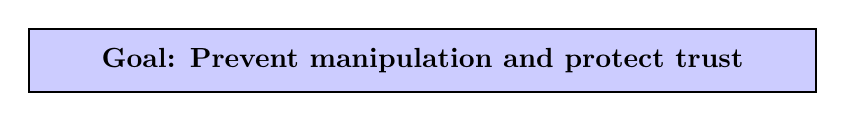
\begin{tikzpicture}
\node[rectangle, draw, thick, fill=blue!20, minimum width=10cm, minimum height=0.8cm, align=center] {\textbf{Goal: Prevent manipulation and protect trust}};
\end{tikzpicture}
\end{center}
\end{frame}

% Slide 14: Deepfakes
\begin{frame}{The Challenge of Deepfakes}
\begin{block}{What are Deepfakes?}
Manipulated videos or audio making it appear that a person said or did things they never actually did
\end{block}

\vspace{0.5cm}

\begin{columns}[T]
\column{0.48\textwidth}
\begin{alertblock}{Risks}
\begin{itemize}
\item Spreading disinformation
\item Damaging reputations
\item Political manipulation
\item Identity fraud
\item Erosion of trust
\end{itemize}
\end{alertblock}

\column{0.48\textwidth}
\begin{exampleblock}{Regulation Requirements}
Deepfakes must be:
\begin{itemize}
\item Explicitly disclosed as such
\item Clearly labeled
\item Identifiable by users
\item Traceable to source
\end{itemize}
\end{exampleblock}
\end{columns}

\vspace{0.5cm}

\begin{center}
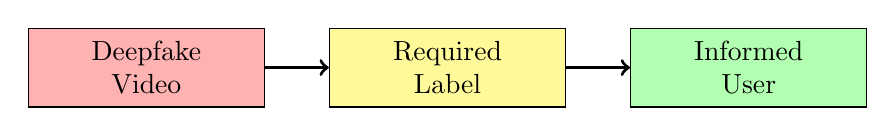
\begin{tikzpicture}[scale=0.85]
\node[rectangle, draw, fill=red!30, minimum width=3cm, minimum height=1cm, align=center] (fake) at (0,0) {Deepfake\\Video};
\node[rectangle, draw, fill=yellow!40, minimum width=3cm, minimum height=1cm, align=center] (label) at (4.5,0) {Required\\Label};
\node[rectangle, draw, fill=green!30, minimum width=3cm, minimum height=1cm, align=center] (user) at (9,0) {Informed\\User};

\draw[->, very thick] (fake) -- (label);
\draw[->, very thick] (label) -- (user);
\end{tikzpicture}
\end{center}

\vspace{0.3cm}
\textbf{Fundamental measure to combat disinformation and protect individuals}
\end{frame}

% Slide 15: General Purpose AI and Foundation Models
\begin{frame}{General Purpose AI and Foundation Models}
\textbf{A new category added during negotiations (Parliament's insistence)}

\vspace{0.4cm}

\begin{block}{What are General Purpose AI Models?}
Systems capable of performing a wide variety of tasks:
\begin{itemize}
\item Generate text, images, code
\item Translate languages
\item Answer questions
\item Analyze data
\end{itemize}
\textbf{Examples:} GPT-4 (OpenAI), Gemini (Google), Claude (Anthropic)
\end{block}

\vspace{0.3cm}

\begin{columns}[T]
\column{0.48\textwidth}
\begin{block}{Key Difference}
Unlike specific-purpose AI:
\begin{itemize}
\item Multi-functional capabilities
\item Broad applicability
\item Potential systemic risks
\end{itemize}
\end{block}

\column{0.48\textwidth}
\begin{block}{Why Regulate Them?}
\begin{itemize}
\item Wide-scale impact
\item Potential for misuse
\item Societal-level risks
\item Need for accountability
\end{itemize}
\end{block}
\end{columns}
\end{frame}

% Slide 16: Systemic Risk Models
\begin{frame}{Models with Systemic Risk}
\textbf{Most powerful models require additional safeguards}

\vspace{0.4cm}

\begin{block}{Identification Threshold}
Models trained with computational power exceeding:
\[10^{25} \text{ FLOPS (Floating Point Operations Per Second)}\]
\vspace{0.2cm}
\small This threshold can be updated by the AI Office as technology evolves
\end{block}

\vspace{0.4cm}

\begin{columns}[T]
\column{0.48\textwidth}
\begin{alertblock}{Systemic Risks}
\begin{itemize}
\item Mass disinformation
\item Coordinated cyberattacks
\item Societal manipulation
\item Large-scale failures
\item Unintended consequences
\end{itemize}
\end{alertblock}

\column{0.48\textwidth}
\begin{block}{Required Obligations}
\begin{itemize}
\item Assess systemic risks
\item Mitigate identified risks
\item Report serious incidents
\item Conduct thorough testing
\item Ensure cybersecurity
\item Report energy consumption
\end{itemize}
\end{block}
\end{columns}
\end{frame}

% Slide 17: Open Source Exception
\begin{frame}{Open Source: Balancing Innovation and Safety}
\begin{columns}[T]
\column{0.48\textwidth}
\begin{block}{Open Source Exemptions}
The regulation recognizes the value of:
\begin{itemize}
\item Collaborative innovation
\item Open-source development
\item Research advancement
\item Community contributions
\end{itemize}
\end{block}

\vspace{0.3cm}

\begin{exampleblock}{Benefits}
Free, open-code models can benefit from lighter requirements
\end{exampleblock}

\column{0.48\textwidth}
\begin{alertblock}{Important Limitation}
Even open-source models must comply with stricter safety obligations if they reach the systemic risk threshold
\end{alertblock}

\vspace{0.3cm}

\begin{block}{The Balance}
\begin{itemize}
\item Encourage innovation
\item Protect against systemic risks
\item Support research community
\item Maintain safety standards
\end{itemize}
\end{block}
\end{columns}

\vspace{0.5cm}

\begin{center}
\textbf{Controversy:} This was one of the most debated aspects\\
\textit{Italy, France, and Germany initially had concerns}
\end{center}
\end{frame}

% Slide 18: Negotiations and Compromises
\begin{frame}{The Path to Agreement: Negotiations}
\begin{tikzpicture}[remember picture,overlay]
\node[anchor=north east, opacity=0.1] at (current page.north east) {\includegraphics[width=0.25\textwidth]{example-image}};
\end{tikzpicture}

\textbf{The regulation on General Purpose AI was highly controversial}

\vspace{0.5cm}

\begin{columns}[T]
\column{0.48\textwidth}
\begin{block}{Initial Concerns}
Italy, France, Germany worried about:
\begin{itemize}
\item Penalizing European companies
\item Competitive disadvantage vs. US/China
\item Over-regulation stifling innovation
\item Compliance costs
\end{itemize}
\end{block}

\vspace{0.3cm}

\begin{block}{Parliament's Position}
Strong regulations needed for:
\begin{itemize}
\item Systemic risk prevention
\item Accountability
\item Transparency
\item Citizen protection
\end{itemize}
\end{block}

\column{0.48\textwidth}
\begin{exampleblock}{The Compromise}
\begin{itemize}
\item Binding obligations for most powerful models
\item Important role for self-regulation through codes of conduct
\item Flexibility for innovation
\item Strong safety requirements maintained
\end{itemize}
\end{exampleblock}

\vspace{0.3cm}

\begin{center}
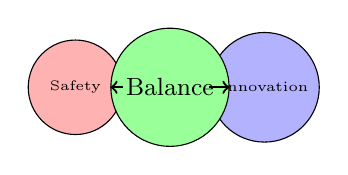
\begin{tikzpicture}[scale=0.8]
\node[circle, draw, fill=red!30, minimum size=1.2cm, font=\tiny] (safety) at (-1.5,0) {Safety};
\node[circle, draw, fill=blue!30, minimum size=1.2cm, font=\tiny] (innov) at (1.5,0) {Innovation};
\node[circle, draw, fill=green!40, minimum size=1.5cm, font=\small] (balance) at (0,0) {Balance};

\draw[->, thick] (safety) -- (balance);
\draw[->, thick] (innov) -- (balance);
\end{tikzpicture}
\end{center}
\end{columns}
\end{frame}

% Slide 19: Sanctions - Part 1
\begin{frame}{Sanctions: Ensuring Compliance}
\textbf{Strong penalties to ensure the regulation is respected}

\vspace{0.5cm}

\begin{block}{Sanction Structure}
Penalties vary based on violation severity and can be calculated as:
\begin{itemize}
\item Fixed amount in millions of euros, OR
\item Percentage of worldwide annual turnover
\end{itemize}
\textbf{Whichever is higher applies}
\end{block}

\vspace{0.5cm}

\begin{center}
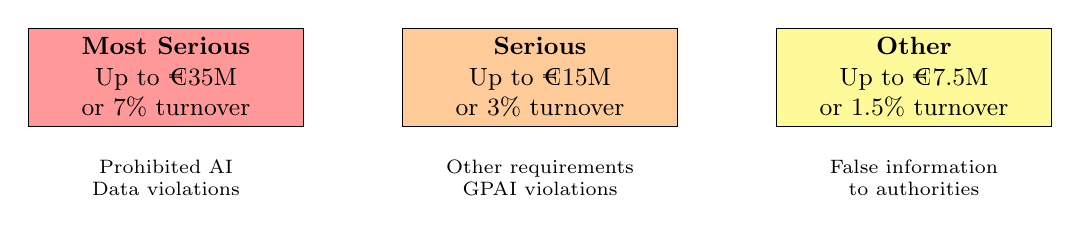
\begin{tikzpicture}[scale=0.95]
% Three tier system
\node[rectangle, draw, fill=red!40, minimum width=3.5cm, minimum height=1.2cm, align=center, font=\small] (tier1) at (0,0) {\textbf{Most Serious}\\Up to €35M\\or 7\% turnover};

\node[rectangle, draw, fill=orange!40, minimum width=3.5cm, minimum height=1.2cm, align=center, font=\small] (tier2) at (5,0) {\textbf{Serious}\\Up to €15M\\or 3\% turnover};

\node[rectangle, draw, fill=yellow!40, minimum width=3.5cm, minimum height=1.2cm, align=center, font=\small] (tier3) at (10,0) {\textbf{Other}\\Up to €7.5M\\or 1.5\% turnover};

\node[below=0.3cm of tier1, text width=3cm, align=center, font=\scriptsize] {Prohibited AI\\Data violations};
\node[below=0.3cm of tier2, text width=3cm, align=center, font=\scriptsize] {Other requirements\\GPAI violations};
\node[below=0.3cm of tier3, text width=3cm, align=center, font=\scriptsize] {False information\\to authorities};
\end{tikzpicture}
\end{center}
\end{frame}

% Slide 20: Sanctions - Part 2
\begin{frame}{Sanctions: Special Provisions}
\begin{columns}[T]
\column{0.48\textwidth}
\begin{block}{SMEs and Startups}
\textbf{Special treatment:}
\begin{itemize}
\item Lower of the two amounts applies
\item Recognition that large fines could be devastating
\item Proportionality principle
\end{itemize}
\end{block}

\vspace{0.3cm}

\begin{exampleblock}{Example}
For an SME violating data requirements:
\begin{itemize}
\item €35M or 7\% turnover
\item \textbf{Lower amount} is applied
\end{itemize}
\end{exampleblock}

\column{0.48\textwidth}
\begin{block}{EU Institutions}
\textbf{No exemptions:}
\begin{itemize}
\item EU agencies subject to fines
\item European Data Protection Supervisor can impose sanctions
\item Rules apply to public and private equally
\end{itemize}
\end{block}

\vspace{0.3cm}

\begin{block}{Citizen Rights}
\begin{itemize}
\item Right to file complaints
\item Market surveillance authorities must investigate
\item Specific procedures guaranteed
\end{itemize}
\end{block}
\end{columns}

\vspace{0.5cm}
\begin{center}
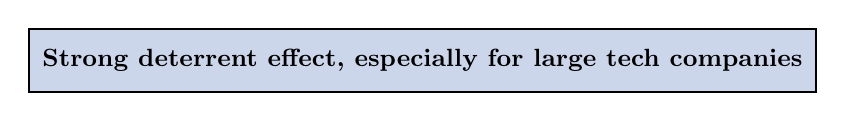
\begin{tikzpicture}
\node[rectangle, draw, thick, fill=euroblue!20, minimum width=10cm, minimum height=0.8cm, align=center, font=\small] {\textbf{Strong deterrent effect, especially for large tech companies}};
\end{tikzpicture}
\end{center}
\end{frame}

% Slide 21: Implementation Timeline
\begin{frame}{When Does It Come Into Effect?}
\textbf{Gradual implementation to allow preparation time}

\vspace{0.5cm}

\begin{center}
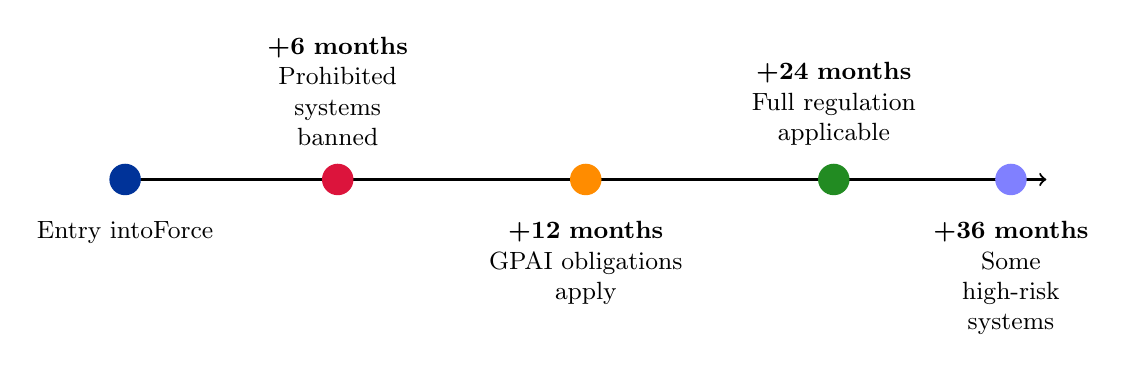
\begin{tikzpicture}[scale=0.9, every node/.style={font=\small}]
% Timeline
\draw[thick, ->] (0,0) -- (13,0);

% Milestones
\node[circle, fill=euroblue, minimum size=0.4cm] (m0) at (0,0) {};
\node[below=0.2cm of m0] {Entry into\\Force};

\node[circle, fill=warningred, minimum size=0.4cm] (m1) at (3,0) {};
\node[above=0.1cm of m1, text width=2cm, align=center] {\textbf{+6 months}\\Prohibited\\systems banned};

\node[circle, fill=cautionorange, minimum size=0.4cm] (m2) at (6.5,0) {};
\node[below=0.2cm of m2, text width=2.5cm, align=center] {\textbf{+12 months}\\GPAI obligations\\apply};

\node[circle, fill=safegreen, minimum size=0.4cm] (m3) at (10,0) {};
\node[above=0.1cm of m3, text width=2.5cm, align=center] {\textbf{+24 months}\\Full regulation\\applicable};

\node[circle, fill=blue!50, minimum size=0.4cm] (m4) at (12.5,0) {};
\node[below=0.2cm of m4, text width=2cm, align=center] {\textbf{+36 months}\\Some high-risk\\systems};
\end{tikzpicture}
\end{center}

\vspace{0.8cm}

\begin{columns}[T]
\column{0.48\textwidth}
\begin{block}{Transition Periods}
\begin{itemize}
\item Companies can prepare
\item Adapt existing systems
\item Train personnel
\item Implement compliance processes
\end{itemize}
\end{block}

\column{0.48\textwidth}
\begin{block}{Existing Systems}
\begin{itemize}
\item Public entities: 4 years for high-risk systems
\item GPAI models: 2 years after obligations apply (3 years total)
\end{itemize}
\end{block}
\end{columns}
\end{frame}

% Slide 22: Global Impact
\begin{frame}{A Model for the World?}
\textbf{The Brussels Effect: EU regulation influences global standards}

\vspace{0.4cm}

\begin{columns}[T]
\column{0.48\textwidth}
\begin{block}{Precedent: GDPR}
The EU's data protection regulation became a de facto global standard:
\begin{itemize}
\item Companies adapted globally
\item Other countries adopted similar laws
\item Set worldwide privacy norms
\end{itemize}
\end{block}

\vspace{0.3cm}

\begin{block}{AI Act Potential}
Could follow the same path:
\begin{itemize}
\item Tech giants must comply for EU market
\item Often easier to apply one standard globally
\item Other jurisdictions may adopt similar frameworks
\end{itemize}
\end{block}

\column{0.48\textwidth}
\begin{block}{Different Approaches}
\textbf{United States:}
\begin{itemize}
\item Market-oriented
\item Less interventionist
\item Sector-specific rules
\end{itemize}

\vspace{0.3cm}

\textbf{China:}
\begin{itemize}
\item Centralized control
\item Social control orientation
\item State-driven development
\end{itemize}

\vspace{0.3cm}

\textbf{European Union:}
\begin{itemize}
\item Rights-based approach
\item Balance protection and innovation
\item "Third way"
\end{itemize}
\end{block}
\end{columns}
\end{frame}

% Slide 23: Open Questions
\begin{frame}{Open Questions and Challenges}
\textbf{The regulation is groundbreaking, but many questions remain}

\vspace{0.5cm}

\begin{enumerate}
\item \textbf{Technological evolution}
   \begin{itemize}
   \item Will rules remain appropriate in 5-10 years?
   \item Can regulation keep pace with AI development?
   \end{itemize}

\item \textbf{Balance between protection and innovation}
   \begin{itemize}
   \item Will Europe fall behind in the global tech race?
   \item Can the EU foster AI champions?
   \end{itemize}

\item \textbf{Enforcement effectiveness}
   \begin{itemize}
   \item Will sanctions be sufficient deterrents?
   \item Do authorities have adequate resources and expertise?
   \end{itemize}

\item \textbf{Global coordination}
   \begin{itemize}
   \item Will other major economies follow suit?
   \item Risk of regulatory fragmentation?
   \end{itemize}

\item \textbf{Practical implementation}
   \begin{itemize}
   \item How will conformity assessment work in practice?
   \item Clarity on edge cases and grey areas?
   \end{itemize}
\end{enumerate}
\end{frame}

% Slide 24: Core Principles
\begin{frame}{Core Principles: The European Choice}
\textbf{The fundamental values guiding the AI Act}

\vspace{0.5cm}

\begin{center}
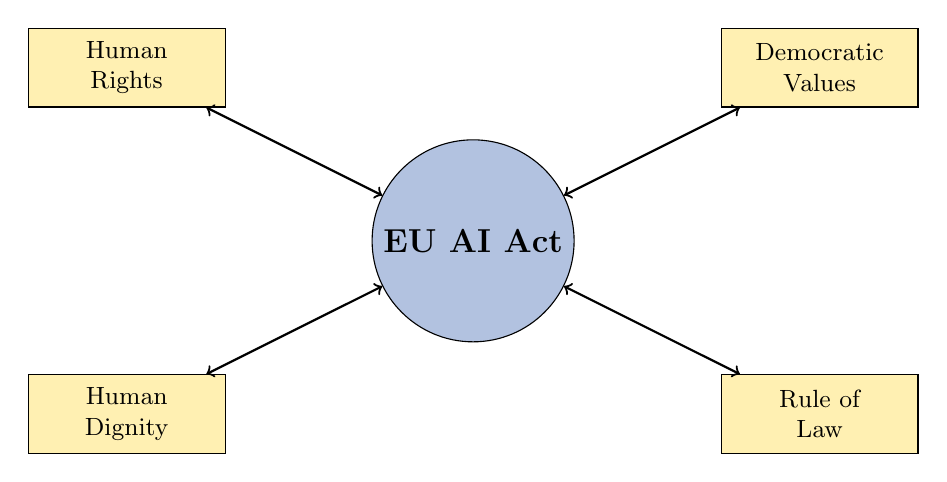
\begin{tikzpicture}[scale=1.1]
% Central node
\node[circle, draw, fill=euroblue!30, minimum size=2.5cm, align=center, font=\large] (center) at (0,0) {\textbf{EU AI Act}};

% Surrounding principles
\node[rectangle, draw, fill=eurogold!30, minimum width=2.5cm, minimum height=1cm, align=center, font=\small] (p1) at (-4,2) {Human\\Rights};

\node[rectangle, draw, fill=eurogold!30, minimum width=2.5cm, minimum height=1cm, align=center, font=\small] (p2) at (4,2) {Democratic\\Values};

\node[rectangle, draw, fill=eurogold!30, minimum width=2.5cm, minimum height=1cm, align=center, font=\small] (p3) at (-4,-2) {Human\\Dignity};

\node[rectangle, draw, fill=eurogold!30, minimum width=2.5cm, minimum height=1cm, align=center, font=\small] (p4) at (4,-2) {Rule of\\Law};

\draw[thick, <->] (center) -- (p1);
\draw[thick, <->] (center) -- (p2);
\draw[thick, <->] (center) -- (p3);
\draw[thick, <->] (center) -- (p4);
\end{tikzpicture}
\end{center}

\vspace{0.5cm}

\begin{center}
\Large \textit{``Technology must serve humanity, not the other way around''}
\end{center}
\end{frame}

% Slide 25: Conclusion
\begin{frame}{Conclusion: A Historic Step Forward}
\begin{columns}[T]
\column{0.55\textwidth}
\begin{block}{Key Achievements}
\begin{itemize}
\item First comprehensive AI regulation worldwide
\item Risk-based, proportionate approach
\item Clear rules on prohibited practices
\item Strong safeguards for high-risk systems
\item Transparency requirements
\item Regulation of powerful AI models
\item Meaningful sanctions
\end{itemize}
\end{block}

\vspace{0.3cm}

\begin{alertblock}{The Challenge}
Making the balance work:
\begin{itemize}
\item Protect fundamental rights
\item Enable innovation
\item Ensure enforcement
\end{itemize}
\end{alertblock}

\column{0.4\textwidth}
\begin{block}{Looking Forward}
\begin{itemize}
\item Implementation will be critical
\item Monitoring needed
\item Adaptation as technology evolves
\item International cooperation
\end{itemize}
\end{block}

\vspace{0.5cm}

\begin{center}
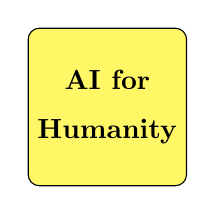
\begin{tikzpicture}
\node[rectangle, draw, fill=yellow!60, rounded corners, minimum size=2cm, align=center, font=\normalsize] {\textbf{AI for}\\[0.2cm]\textbf{Humanity}};
\end{tikzpicture}
\end{center}
\end{columns}

\vspace{0.5cm}

\begin{center}
\large \textbf{In an algorithm-driven world, clear rules are essential\\to ensure AI truly serves humanity}
\end{center}
\end{frame}

% Final slide
\begin{frame}
\begin{center}
\Huge Thank You!

\vspace{1cm}

\Large Questions?

\vspace{1.5cm}

\normalsize
\textbf{IIS Fermi Sacconi Ceci}\\
Ascoli Piceno, Italy

\vspace{0.5cm}

\textit{Understanding AI Regulation\\for a Better Digital Future}
\end{center}
\end{frame}

\end{document}
